\chapter{Introduction}

\section{Purpose}


The \textit{Students\&Companies (S\&C)} platform bridges the gap between university students seeking
internships and companies offering them. It simplifies the process of matching students with internship
opportunities based on their skills, experiences, and preferences, as well as companies' requirements
and offered benefits.

The software involves three main actors: \textbf{students}, \textbf{companies}, and \textbf{universities}.

\begin{itemize}
    \item \textbf{Students} use the platform to search and apply for internships, submit their CVs, and
    receive recommendations tailored to their profiles.
    \item \textbf{Companies} advertise internships, specify requirements, and manage the selection
    process for suitable candidates.
    \item \textbf{Universities} monitor the execution of internships and handle complaints or
    issues that may arise.
\end{itemize}

S\&C features a \textbf{recommendation system} that matches students and internships using mechanisms
ranging from keyword-based searches to advanced statistical analyses. The platform also facilitates
communication, supports the selection process, and tracks internship progress to ensure transparency
for all involved parties.

\newpage
\section{Scope}

The Students\&Companies (S\&C) platform is a web application designed to facilitate communication and
matchmaking between university students seeking internships and companies offering them. The platform
simplifies and automates the process by enabling students to explore and apply for internships, while
also allowing companies to advertise their openings and identify suitable candidates. Additionally,
a sophisticated recommendation system enhances the user experience by automatically suggesting relevant
matches to both students and companies based on their preferences and requirements.

This document aims to outline the key architectural decisions behind the design and implementation of
the S\&C platform. Given the diverse user base, which includes students, companies, and universities,
and the need for simultaneous interaction among these parties, a web application was chosen as the
foundation. Its accessibility and ease of use ensure a seamless experience for users across various
locations and devices.

The complexity of the platform, along with the distinct functionalities it provides—such as recommendations,
selection processes, and feedback collection—led to the choice of a microservices architecture.
This architectural style was selected due to its ability to offer scalability, flexibility, resilience,
and modularity. Each microservice operates independently, allowing for targeted scaling based on
demand, individual updates and deployments, and clear separation of responsibilities.
The result is a system that is both maintainable and adaptable to evolving requirements.

From a deployment perspective, the system adopts a three-tier architecture. The user client
layer represents the web and mobile interfaces used by students, companies, and universities.
The server layer hosts all microservices, which manage the business logic and application
functionality. Finally, the shared database layer ensures consistency in data storage,
maintaining information about users, internships, recommendations, and feedback.

To manage interactions between microservices, the platform uses a combination of communication
patterns based on specific functional needs. For real-time or asynchronous interactions, an
event-driven communication model is employed. In this approach, some microservices act as event
publishers while others function as consumers. For example, the Notification Microservice processes
events related to complaints, messages, and new recommendations, while other services publish events
to reflect changes in system states, such as the pubblication of a new message on the communication platform
or the acceptance of a student for an interview.
 
For functionalities that do not require immediate interactions, synchronous communication mechanisms
are used. This includes scenarios such as retrieving a list of internships or submitting CVs, where
sequential processing and immediate feedback are necessary. The combination of event-driven and
synchronous communication ensures that the system remains both responsive and straightforward to
use, catering to the dynamic needs of its users.

All these architectural choices are just mentioned here to provide an overview of the system; they
will be better explained and unpacked down the line of this document. The following image shows
the major components of the Students\&Companies system.
\newline
\newline

\begin{figure} [H]
    \centering
    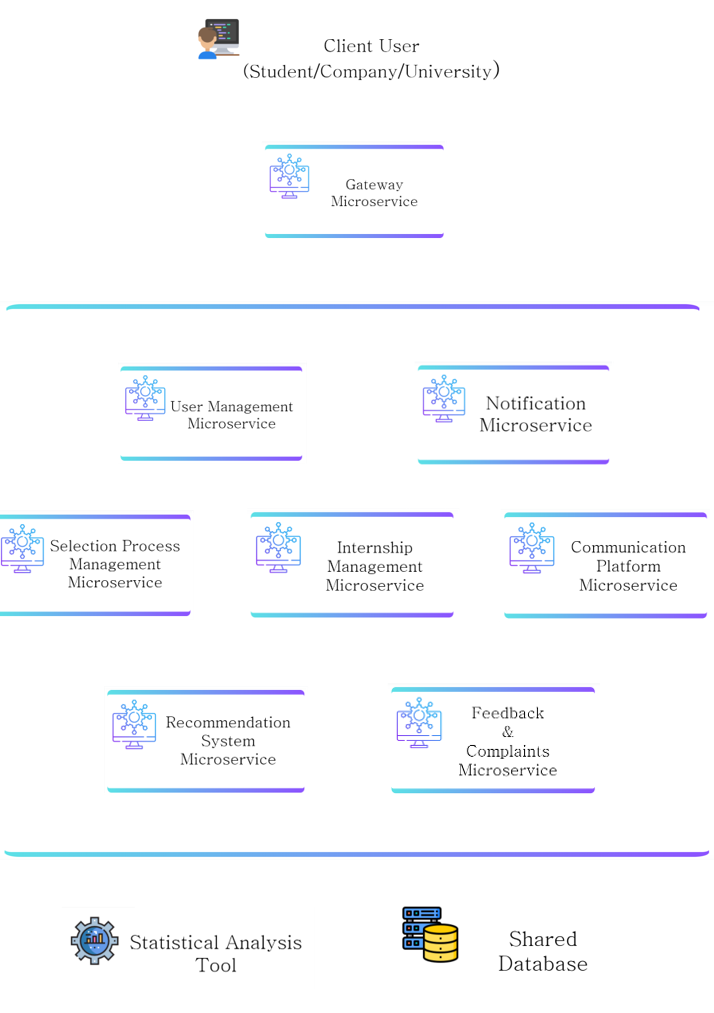
\includegraphics [width=0.75\linewidth] {microservice.png}
\end{figure}


\newpage
\section{Definitions, Acronyms, Abbreviations}
\subsection{Definitions}

A brief list of the most meaningful and relevant terms and synonyms used in this document is reported
here, in order to make reading process smoother and clearer:

\begin{longtable}{p{0.50\textwidth}p{0.50\textwidth}}
    \textbf{\large Term} & \textbf{\large Definition} \\
    \vspace{0.5em}\\
    \hline
    \vspace{0.5em}\\
    \endfirsthead
    \textbf{\large Term} & \textbf{\large Description} \\
    \vspace{0.5em}\\
    \hline
    \vspace{0.5em}\\
    \endhead
    
    Internship, Placement, Work-Experience & A temporary work opportunity offered by a company, designed
    for students to gain practical experience in a professional environment while applying their academic
    knowledge. \\
    \vspace{0.5em}\\
    CV, Resume & A document created by a student containing their personal information, skills,
    educational background, and work experience, used to apply for internships or jobs. \\
    \vspace{0.5em}\\
    Recommendation System, Suggestion System & A feature of the platform that identifies and matches
    suitable internships for students or suitable candidates for companies based on their profiles,
    preferences, and requirements. \\
    \vspace{0.5em}\\
    Student Profile & A digital representation of a student within the system, containing personal
    details, uploaded CVs, skills. \\
    \vspace{0.5em}\\
    Company Profile & A digital representation of a company within the system, containing details
    about the company, uploaded projects or internships. \\
    \vspace{0.5em}\\
    Recommendation Process & The sequence of steps executed by the system to align the skills and
    preferences of students with the requirements of available internships offered by companies. \\
    \vspace{0.5em}\\
    Feedback, Suggestions & Information collected from students and companies
    during the selection process and the internship to refine the matching system and improve user satisfaction. \\
    \vspace{0.5em}\\
    Communication Space, Chat Feature, Messaging System & A feature in the platform that allows
    students, companies, and universities to interact and share important updates or resolve concerns. \\
    \vspace{0.5em}\\
    Selection Process & A phase in which companies evaluate student applications, conduct
    interviews, and finalize the selection of candidates for internships. \\
    \vspace{0.5em}\\
    Interview Setup, Interview Management & The process supported by the system to schedule,
    conduct, and manage interviews between companies and students. \\
    \vspace{0.5em}\\
    Monitoring by University & The process where the university oversees the activities and
    outcomes of student internships and intervenes if necessary. \\
    \vspace{0.5em}\\
    Complaint Resolution & The process of identifying and addressing issues raised by students
    or companies during or after the internship period. \\
    \vspace{0.5em}\\
    Submission Deadline, Application Deadline & The last date for students to submit applications
    for an internship or for companies to post available projects on the platform. \\
    \vspace{0.5em}\\
    Notification System, Alert System & A functionality in the platform that keeps users informed
    about new opportunities, deadlines, or important events. \\
    \vspace{0.5em}\\
    Platform, System, Application & All synonyms for the software platform being developed to
    manage the interactions and processes related to internships. \\
    \vspace{0.5em}\\
    Statistical Analysis & The process by which the system evaluates collected feedback and
    interactions to improve its recommendation algorithms and user experience. \\

    \vspace{0.5em}\\
    Architectural Style & A way of designing a system that defines general principles and patterns for how different
    parts should interact and be organized. \\
    
    \vspace{0.5em}\\
    Structure/View & A representation of a system that highlights specific aspects, such as how components are connected,
    how they interact, or how they are distributed across different locations. \\
    
    \vspace{0.5em}\\
    Component & An independent part of a system that performs a specific function and can often be reused in different
    systems or contexts. \\
    
    \vspace{0.5em}\\
    API & A set of rules and tools that allow different software programs to communicate and share information or
    functionality with each other. \\
    
    \vspace{0.5em}\\
    RESTful API & A type of API that uses standard web protocols like HTTP to let systems access and manipulate resources,
    following specific guidelines for simplicity and scalability. \\
    
    \vspace{0.5em}\\
    Web Application & A program accessed through a web browser that combines client-side and server-side resources to
    provide interactive features and services. \\
    
    \vspace{0.5em}\\
    Microservice & A design approach where a system is divided into small, self-contained services that handle specific
    tasks and can be developed, deployed, and updated independently. \\
    
    \vspace{0.5em}\\
    Three-tier architecture & A system divided into three parts: one for displaying information to users (presentation),
    one for processing logic (application), and one for managing and storing data (database). \\
    
    \vspace{0.5em}\\
    Event-Driven Architecture & A system where actions are triggered by events, such as a notification being sent when
    a user performs a specific action. \\
    
    \vspace{0.5em}\\
    Synchronous communication among microservices & A communication method where one service sends a request to another
    and waits for the response before continuing. \\
    
    \vspace{0.5em}\\
    Asynchronous communication among microservices & A communication method where one service sends a request and does
    not wait for a response, allowing the system to handle tasks more flexibly. \\
    
\end{longtable}

\subsection{Acronyms}

A list of acronyms used throughout the document for simplicity and readability:
\\
\begin{itemize}
    \item {RASD} - Requirements Analysis and Specification Document
    \item {DD} - Design Document
    \item {S\&C} - Students \& Companies
    \item {API} - Application Programming Interface
    \item {UI} - User Interface
    \item {UML} - Unified Modeling Language
    \item {DB} - Database
    \item {DBMS} - Database Management System
\end{itemize}

\newpage
\section{Reference Documents} 

Here’s a list of reference documents that have been used in order to shape the Design Document of the \textit{Students\&Companies} system. In the following, all external sources of information that have contributed to the design of this document are mentioned.

\begin{enumerate}
    \item Stakeholders’ specification provided by the R\&DD assignment for the Software Engineering II course at Politecnico Di Milano for the year 2024/2025.
    \item ``29148-2018, ISO/IEC/IEEE International Standard, Systems and software engineering, Life cycle processes, Requirements engineering'', by IEEE, 2018. \\
    Link: \url{https://ieeexplore.ieee.org/document/8559686}
    \item UML specifications, version 2.5.1. \\
    Link: \url{https://www.omg.org/spec/UML/2.5.1/About-UML}
    \item Alloy documentation, version 6.1.0.8. \\
    Link: \url{https://alloy.readthedocs.io/en/latest/}
\end{enumerate}

\newpage
\section{Document Structure}
The Design Document for the Student\&Company project are organized into five primary parts: the first
is the introduction, while the remaining four each focus on a specific aspect of the system's overall design,
which will
help facilitate the development and final implementation of the product.

The \textbf{Introduction} serves to
provide a concise overview of the project, detailing the objectives and goals that are to be accomplished
through its development, as outlined earlier in the RASD.

Moving on, Section 2, titled \textbf{Architectural Design},
is the most critical design-related section and aims to present the software architecture of Student\&Company
through various views and structural representations. This section is divided into multiple parts: 

The first part, Overview, delivers a high-level summary of the core components of the system and how
they interact with each other, explained in an informal notation that makes the structure more accessible.

The second part, Component View, presents the first of the architectural structures, the Component \&
Connector structure, which is crucial for demonstrating the system’s components from a dynamic perspective
and the way in which they collaborate to meet the final objectives; it largely uses UML component diagrams
to convey these interactions.

The Deployment View, the third part, focuses on the deployment structure of
Student\&Company, illustrating how the software components correspond to the physical hardware that will
run the application. The mapping between the software and hardware is illustrated with UML deployment
diagrams, which are extremely helpful in visualizing this relationship.

Then, the Runtime View follows,
employing sequence diagrams to describe the flow of events and interactions within the system’s
components, ensuring consistency with the previously discussed sections.

The Component Interfaces
section comes next, where a detailed specification of the important methods and functions exposed
by each interface of the system’s components is provided, making sure to cover all relevant aspects.

The final part of Section 2 discusses the Selected Architectural Styles and Patterns, offering a
review of the primary architectural styles and patterns, followed by a detailed explanation of why
they were selected for this particular project.

Section 3, on \textbf{User Interface Design}, shifts focus to the design of user interfaces (UI), offering
guidelines for UI designers on how the final application should appear, including color schemes,
the placement of key UI elements, and also the logical role that these interfaces play in the
development process, clarifying what functionalities they provide to the user.

Following this,
Section 4, which covers \textbf{Requirement Traceability}, provides a matrix that clearly shows how the
requirements for Student\&Company, which were previously drawn up, map onto the components discussed
in earlier sections of the document, ensuring that all requirements are adequately addressed by the
system.

Finally, Section 5, \textbf{Implementation, Integration, and Test Plan}, explains the strategy for
implementing the system, detailing the order in which the components will be developed, the
approach for integrating new sub-components into the application as it progresses, and the
testing strategy to ensure that all components work seamlessly together within the system.